% =========================================================
% 3.10.3 Full Adder
% =========================================================

\subsection{পূর্ণযোগক (\textenglish{Full Adder})}

অর্ধযোগক (\textenglish{Half Adder}) দুটি ১-বিট বাইনারি সংখ্যা যোগ করতে পারে, কিন্তু
পূর্ববর্তী ধাপ থেকে কোনো \textenglish{carry} ইনপুট হিসেবে গ্রহণ করতে পারে না।
বাস্তবে বহু-বিট বাইনারি সংখ্যা যোগ করার সময় আগের ধাপের \textenglish{carry}
পরবর্তী ধাপে যুক্ত করতে হয়। এই সমস্যা সমাধানের জন্য পূর্ণযোগক ব্যবহার করা হয়।

যে সমন্বিত লজিক সার্কিট তিনটি ১-বিট বাইনারি ইনপুট যোগ করে
যোগফল (\textenglish{Sum}) এবং ক্যারি আউট (\textenglish{Carry-out})
নির্ণয় করে, তাকে পূর্ণযোগক (\textenglish{Full Adder}) বলে।

পূর্ণযোগকের তিনটি ইনপুট হলো—
\[
A,\;B,\;C_i
\]
এখানে \(C_i\) হলো পূর্ববর্তী ধাপ থেকে আগত \textenglish{carry-in}।

এটির দুটি আউটপুট হলো—
\[
S \quad \text{এবং} \quad C_o
\]
যেখানে \(S\) হলো \textenglish{Sum} এবং \(C_o\) হলো \textenglish{Carry-out}।

\smallskip

উদাহরণ হিসেবে,
\[
1+1+0=10
\]
এখানে \textenglish{sum} হবে \(0\) এবং \textenglish{carry} হবে \(1\)।

আবার,
\[
1+1+1=11
\]
এখানে \textenglish{sum} হবে \(1\) এবং \textenglish{carry} হবে \(1\)।

\par\begingroup

\textbf{মনে রাখবে:}
অর্ধযোগকে ২টি ইনপুট থাকে, কিন্তু পূর্ণযোগকে ৩টি ইনপুট থাকে।
এই অতিরিক্ত ইনপুটটি হলো \(C_i\), যা পূর্ববর্তী ধাপের \textenglish{carry} বহন করে।
\par\endgroup


% =========================================================
% Full Adder Box Image
% =========================================================

\begin{center}
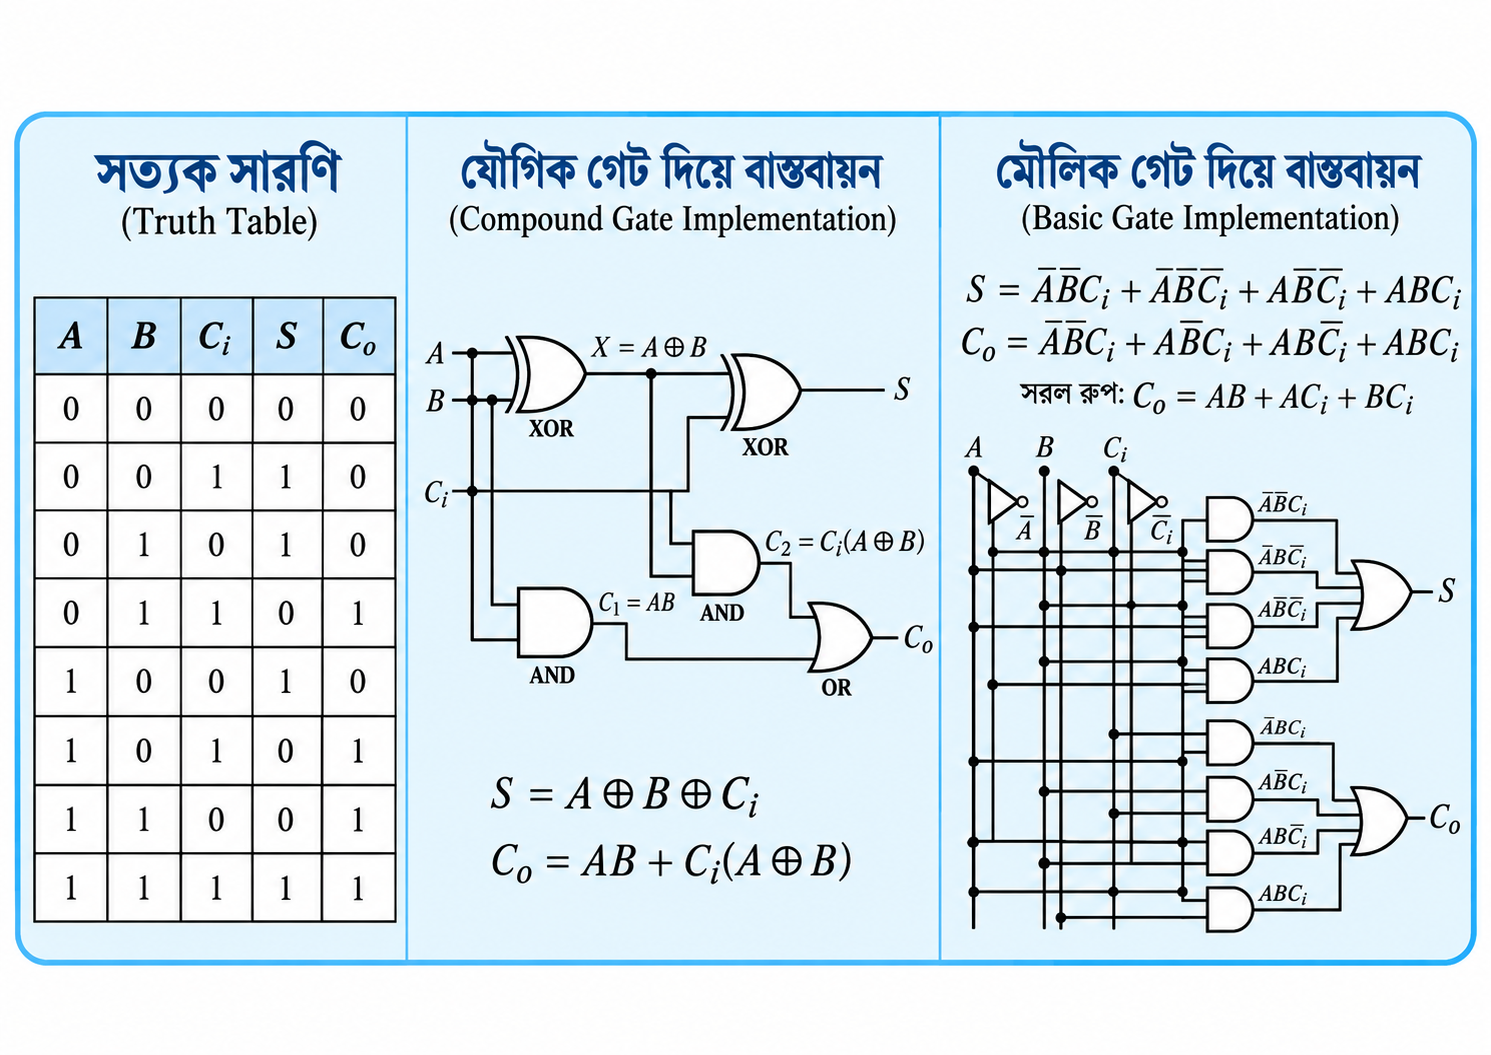
\includegraphics[width=\textwidth]{chapters/Chapter03/resources/images/full_adder_box.png}

\smallskip
{\small \textbf{চিত্র:} পূর্ণযোগকের সত্যক সারণি, যৌগিক গেট দিয়ে বাস্তবায়ন এবং মৌলিক গেট দিয়ে বাস্তবায়ন}
\end{center}

% =========================================================
% Boolean expressions of Full Adder
% =========================================================

\paragraph{যোগফল \(S\)-এর বুলিয়ান রাশি নির্ণয়:}

সত্যক সারণি থেকে দেখা যায়, \(S=1\) হয় নিম্নোক্ত ইনপুটের জন্য:
\[
001,\;010,\;100,\;111
\]

অতএব,
\[
\begin{aligned}
S &=
\overline{A}\,\overline{B}\,C_i
+\overline{A}\,B\,\overline{C_i}
+A\,\overline{B}\,\overline{C_i}
+A\,B\,C_i \\[4pt]
&=
\overline{A}\left(\overline{B}C_i+B\overline{C_i}\right)
+A\left(\overline{B}\,\overline{C_i}+BC_i\right) \\[4pt]
&=
\overline{A}(B\oplus C_i)+A\overline{(B\oplus C_i)} \\[4pt]
&=
A\oplus(B\oplus C_i) \\[4pt]
&=
A\oplus B\oplus C_i
\end{aligned}
\]

সুতরাং,
\[
\boxed{S=A\oplus B\oplus C_i}
\]

\paragraph{ক্যারি \(C_o\)-এর বুলিয়ান রাশি নির্ণয়:}

সত্যক সারণি থেকে দেখা যায়, \(C_o=1\) হয় নিম্নোক্ত ইনপুটের জন্য:
\[
011,\;101,\;110,\;111
\]

অতএব,
\[
\begin{aligned}
C_o &=
\overline{A}BC_i
+A\overline{B}C_i
+AB\overline{C_i}
+ABC_i \\[4pt]
&=
\overline{A}BC_i
+A\overline{B}C_i
+AB(\overline{C_i}+C_i) \\[4pt]
&=
\overline{A}BC_i
+A\overline{B}C_i
+AB \\[4pt]
&=
C_i(\overline{A}B+A\overline{B})+AB \\[4pt]
&=
C_i(A\oplus B)+AB
\end{aligned}
\]

অর্থাৎ,
\[
\boxed{C_o=AB+C_i(A\oplus B)}
\]

এখন এটিকে আরও পরিচিত রূপে লেখা যায়—
\[
\begin{aligned}
C_o &= AB+C_i(A\oplus B) \\[4pt]
&= AB+C_i(\overline{A}B+A\overline{B}) \\[4pt]
&= AB+\overline{A}BC_i+A\overline{B}C_i \\[4pt]
&= AB+BC_i+AC_i
\end{aligned}
\]

সুতরাং,
\[
\boxed{C_o=AB+AC_i+BC_i}
\]

\par\begingroup

\textbf{পূর্ণযোগকের দুটি গুরুত্বপূর্ণ সূত্র:}
\[
S=A\oplus B\oplus C_i
\]
\[
C_o=AB+C_i(A\oplus B)
\]
অথবা,
\[
C_o=AB+AC_i+BC_i
\]
\par\endgroup


% =========================================================
% 3.10.4 Full Adder using two Half Adders
% =========================================================

\subsubsection*{অর্ধযোগক ও পূর্ণযোগকের পার্থক্য}

\begin{center}
\renewcommand{\arraystretch}{1.35}
\begin{tabular}{|p{0.20\linewidth}|p{0.34\linewidth}|p{0.34\linewidth}|}
\hline
\rowcolor{gray!15}
\textbf{বিষয়} & \textbf{অর্ধযোগক (\textenglish{Half Adder})} & \textbf{পূর্ণযোগক (\textenglish{Full Adder})} \\
\hline
ইনপুট সংখ্যা & ২টি & ৩টি \\
\hline
ইনপুট & \(A,B\) & \(A,B,C_i\) \\
\hline
ক্যারি ইনপুট & নেই & আছে \\
\hline
আউটপুট & \(S,C\) & \(S,C_o\) \\
\hline
ব্যবহার & দুটি ১-বিট সংখ্যা যোগ করে & ক্যারিসহ দুটি ১-বিট সংখ্যা যোগ করে \\
\hline
গঠন & \textenglish{XOR} ও \textenglish{AND} গেট & \textenglish{XOR}, \textenglish{AND} ও \textenglish{OR} গেট \\
\hline
\end{tabular}
\end{center}

% =========================================================
% 3.10.6 Applications
% =========================================================

\subsubsection*{অ্যাডারের ব্যবহার}

অ্যাডার ডিজিটাল ইলেকট্রনিক্স ও কম্পিউটার ব্যবস্থায় অত্যন্ত গুরুত্বপূর্ণ।
এর কয়েকটি ব্যবহার হলো—

\begin{enumerate}
    \item \textenglish{ALU} (\textenglish{Arithmetic Logic Unit})-তে বাইনারি যোগের কাজে।
    \item বহু-বিট বাইনারি সংখ্যা যোগ করতে।
    \item কম্পিউটার প্রসেসরের গাণিতিক অংশে।
    \item ডিজিটাল ক্যালকুলেটরে।
    \item বিভিন্ন ডিজিটাল সার্কিটে \textenglish{sum} ও \textenglish{carry} নির্ণয়ে।
\end{enumerate}

\par\begingroup

\textbf{পরীক্ষার জন্য খুব গুরুত্বপূর্ণ:}
\begin{itemize}[label={{\bulletfont\textbullet}}, leftmargin=*, nosep]
    \item \textbf{Half Adder:}
    \[
    S=A\oplus B,\qquad C=AB
    \]

    \item \textbf{Full Adder:}
    \[
    S=A\oplus B\oplus C_i
    \]
    \[
    C_o=AB+C_i(A\oplus B)
    \]
    অথবা,
    \[
    C_o=AB+AC_i+BC_i
    \]
\end{itemize}
\par\endgroup
